\documentclass[times]{elsarticle}


\usepackage[dvipsnames]{xcolor}
\usepackage{amsmath}
\usepackage{amsfonts}
\usepackage{amssymb}
\usepackage{lineno}
\usepackage{enumerate}
\usepackage{times}
\usepackage{subcaption}
\usepackage{graphicx,psfrag}
\usepackage{pgfplotstable}
\usepackage[skip=0pt]{caption}


\newcommand\solidrule[1][0.25cm]{\rule[0.5ex]{#1}{1pt}}
\newcommand\dashedrule{\mbox{%
  \solidrule[2mm]\hspace{2mm}\solidrule[2mm]}}

\newcommand{\dotrule}[1]{%
	\parbox{#1}{\dotfill}} 

\makeatletter
\newcommand \Dotfill {\leavevmode \cleaders \hb@xt@ .22em{\hss .\hss }\hfill \kern \z@}
\makeatother
 
\newcommand{\Dotrule}[1]{%
   \parbox{#1}{\Dotfill}} 

\begin{document}

\title{Behaviour of the Serre Equations in the Presence of Steep Gradients Revisited}

\author[ANU]{J.P.A.~Pitt\corref{cor1}}
\ead{jordan.pitt@anu.edu.au }
\author[ANU]{C.~Zoppou}
\ead{christopher.zoppou@anu.edu.au}
\author[ANU]{S.G.~Roberts}
\ead{stephen.roberts@anu.edu.au}

\cortext[cor1]{Corresponding author}
\address[ANU]{Mathematical Sciences Institute, Australian National University, Canberra, ACT 0200, Australia}
 \begin{abstract}

 \end{abstract}	
 
  \begin{keyword}
  	Serre equations\sep steep gradients \sep dam break
  \end{keyword}
  
 \maketitle
\linenumbers
%--------------------------------------------------------------------------------

\section{Serre Equations}
\label{section:Serre Equations}
The Serre equations can be derived by integrating the full incompressible Euler equations over the water depth \cite{Su-Gardener-1969-536}. They can also be derived as an asymptotic expansion of the Euler equations \cite{Bonneton-Lannes-2009-16601}. 

Assuming a constant horizontal bed the one-dimensional Serre equations are \cite{Guyenne-etal-2014-169}
\begin{linenomath*}
\begin{subequations}\label{eq:Serre_nonconservative_form}
\begin{gather}
\dfrac{\partial h}{\partial t} + \dfrac{\partial (uh)}{\partial x} = 0
\label{eq:Serre_continuity}
\end{gather}
and
\begin{gather}
\underbrace{\underbrace{\dfrac{\partial (uh)}{\partial t} + \dfrac{\partial}{\partial x} \left ( u^2h + \dfrac{gh^2}{2}\right )}_{\text{Shallow Water Wave Equations}} + \underbrace{\dfrac{\partial}{\partial x} \left (  \dfrac{h^3}{3} \left [ \dfrac{\partial u }{\partial x} \dfrac{\partial u}{\partial x} - u\dfrac{\partial^2 u}{\partial x^2}  - \dfrac{\partial^2 u}{\partial x \partial t}\right ] \right )}_{\text{Dispersion Terms}} = 0.}_{\text{Serre Equations}}
\label{eq:Serre_momentum}
\end{gather}
\end{subequations}
\end{linenomath*}
Where $u(x,t)$ is the  horizontal velocity over the depth of water $h(x,t)$, $g$ is the acceleration due to gravity, $x$ is the horizontal spatial variable and $t$ is time. 

The Serre equations are conservation laws for mass ($h$) and momentum ($uh$) \cite{Su-Gardener-1969-536}. The Serre equations admit a Hamiltonian \cite{Li-Y-2002,Green-Naghdi-1976-237}
\begin{linenomath*}
	\begin{gather}
	\label{eqn:Hamildef}
	\mathcal{H}(x,t) = \frac{1}{2} \left(hu^2 + \frac{h^3}{3} \left(\frac{\partial u}{\partial x}\right)^2 + gh^2\right)
	\end{gather}
\end{linenomath*}
which represents the energy for the Serre equations and is also conserved.

The total amount of a quantity $q$ in a system occurring on the interval $[a,b]$ is measured by
\begin{linenomath*}
\begin{gather*}
\label{eqn:Condef}
\mathcal{C}_q(t) = \int_{a}^{b} q(x,t)\, dx .
\end{gather*}
\end{linenomath*}
Conservation of a quantity $q$ implies that $\mathcal{C}_{q}(0) = \mathcal{C}_{q}(t)$ $\forall t$ provided the interval is fixed and the system is closed. Our numerical methods should have this conservation property for $h$, $uh$ and $\mathcal{H}$.  


%--------------------------------------------------------------------------------
\section{Smoothed Dam Break Problem}
\label{section:smootheddambreak}
%--------------------------------------------------------------------------------
%put background in here more on the rerasion for doing this smoothing
In the literature the dam-break problem is approximated by a smooth hyperbolic tangent function \cite{Mitsotakis-etal-2014,Mitsotakis-etal-2017}. Such an approximation is called a smoothed dam-break problem and is defined by
\begin{linenomath*}
\begin{subequations}
\begin{gather}
h(x,0) = h_0 + \frac{h_1 - h_0}{2}\left(1 + \tanh\left(\frac{x_0 - x}{\alpha}\right)\right),
\end{gather}
\begin{gather}
u(x,0) = 0.0m/s
\end{gather}
\label{eq:sdbi}
\end{subequations}
\end{linenomath*}
where $\alpha$ measures the distance over which approximately $46\%$ of the smooth transition between the two heights of $h_0$ and $h_1$ centred around $x_0$ occurs. Decreasing $\alpha$ increases the steepness of the smoothed dam-break problem as can be seen in Figure \ref{fig:dbsmoothinit} by varying $\alpha$ for different smoothed dam-break problems with fixed heights $h_1 =1.8m$ and $h_0 = 1m$ and fixed centre $x_0 = 500m$. These are the same $h_0$ and $h_1$ values as those of the dam-break problems of \citet{El-etal-2006} and \citet {Hank-etal-2010-2034} and will be the values used in Sections \ref{section:smootheddambreak} and \ref{section:NumRes}.
\begin{figure}
\centering
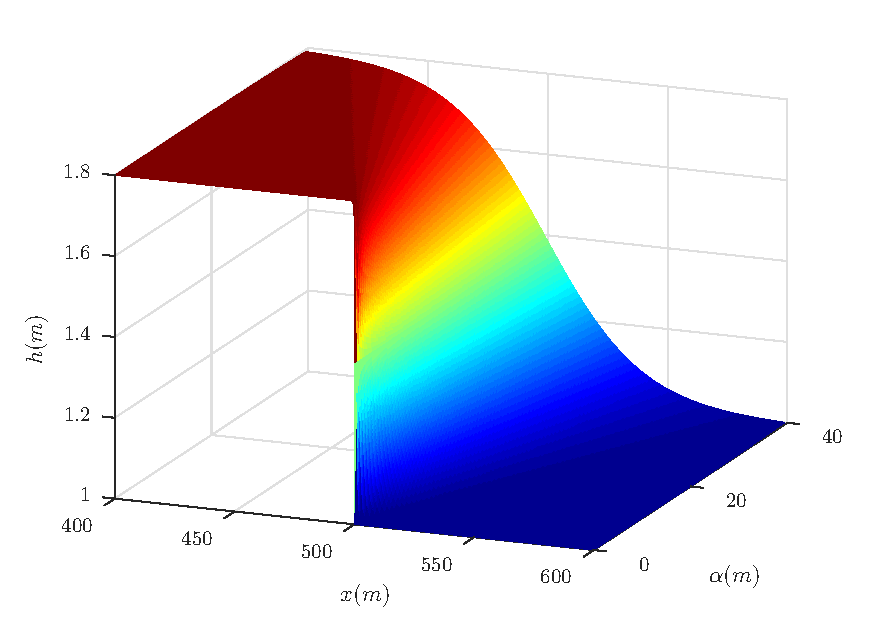
\includegraphics[width=0.6\textwidth]{pics/explainers/dbs.pdf}
\caption{Initial conditions for the smooth dam-break problem with $h_0 = 1m$, $h_1 = 1.8m$ and $x_0 =500m$ as $\alpha$ varies.}
\label{fig:dbsmoothinit}
\end{figure}
%
\subsection{Assessing validity of Numerical Solutions}
There are no analytic results for the Serre equations for either the discontinuous dam-break problem or its smoothed approximation. To assess the validity of our numerical solutions we use four comparisons. The first two investigate the behaviour of the numerical solutions of our highest order method as $\Delta x \rightarrow 0$ by measuring the relative distance between solutions ($L_1$) and the error in conservation ($C_1$). The third compares the numerical solutions of different methods when $\Delta x$ is fixed. Lastly there are also the Whitham modulation results of \citet{El-etal-2006} who derived an expression for the amplitude of the leading wave of an undular bore. If our numerical solutions converged with small errors in conservation as $\Delta x \rightarrow 0$, agree with numerical solutions from different methods and agree with the Whitham modulation results then our numerical solutions are accurate approximate solutions of the Serre equations. 

To compare the numerical solutions requires some notation around the spatial grids defined by $x_i$ and the temporal grids defined by $t^n$ upon which the numerical solutions are calculated. Firstly these grids are uniform so that $\Delta x = x_{i} - x_{i-1}$ $\forall i$ and $\Delta t = t^{n} - t^{n-1}$ $\forall n$ are both constant. Secondly subscripts and superscripts are used to denote where a quantity $q$ is evaluated in the following way $q_i^n = q(x_i,t^n)$. Lastly a cell is a particularly useful unit of the finite volume method, where the $i$th cell is the interval [$x_i -\Delta x/2$,$x_i +\Delta x/2$] centred around $x_{i}$. 

\subsubsection{Distance between Numerical Results}
By measuring the relative distance between numerical solutions we can assess whether our numerical solutions are converging as $\Delta x  \rightarrow 0$. Rather than comparing all numerical results to one another all numerical solutions are compared to the one with the smallest $\Delta x$. In these experiments $\Delta x$ was lowered by dividing it by $2$ thus the grid built from the smallest $\Delta x$ contains all the locations $x_i$ in the grid built from the larger $\Delta x$ values. To measure the relative distance between quantities on these grids we compare them only on the common points $x_i$ in the larger $\Delta x$ grid. So that for some quantity $q$ we have our numerical approximation to it on the grid built from the smallest $\Delta x$ $q^*$ and on the grid built from the grid larger $\Delta x$ $q'$ with the relative distance between the two being
\begin{linenomath*}
	\begin{gather}
	L_1^{q} = \dfrac{\sum_{i} \left| q'(x_i)  - q^*(x_i)\right|}{\sum_{i} \left| q^*(x_i)\right|}.
	\label{eq:L1def}
	\end{gather}
\end{linenomath*}

\subsubsection{Conserved Quantities}
The initial conditions of the smoothed dam-break \eqref{eq:sdbi} were integrated to get the following expressions for $C_{h}(0)$, $C_{uh}(0)$ and $C_{\mathcal{H}}(0)$ provided $x_0$ is the midpoint of the spatial domain $\left[a,b \right]$ in which the smoothed dam-break occurs
\begin{linenomath*}
	\begin{subequations}
		\begin{gather*}
		\mathcal{C}_{h}(0) = \frac{h_1 + h_0}{2}\left(b- a\right),
		\label{eq:Chdef}
		\end{gather*}
		\begin{gather*}
		\mathcal{C}_{uh}(0) = 0
		\label{eq:Cuhdef}
		\end{gather*}
		and
		\begin{gather*}
		\mathcal{C}_{\mathcal{H}}(0) = \frac{g}{4} \left(h_0^2 - h_1^2 + \alpha\left(h_1 - h_0\right)^2\tanh\left(\frac{a - b}{2 \alpha}\right)\right).
		\label{eq:CHdef}
		\end{gather*}
		\label{eq:Canalyticvalues}	
	\end{subequations}
\end{linenomath*}

To calculate the total amount of a quantity $q$ in our numerical solution we fit a quartic interpolant of the primitive variables $h$ and $u$ over a cell utilising quantities from neighbouring cells and then apply Gaussian quadrature with 3 points to get a good approximation to the total amount of $q$ in a cell. The amounts of $q$ in each cell are summed across all cells to get the total amount of $q$ in the domain at time $t$ which we call $\mathcal{C^*}_{q}(t)$. The error in conservation of a quantity $q$ for a numerical method is
\begin{linenomath*}
	\begin{gather}
	C_1^q = \frac{\left| \mathcal{C}_{q}(0) - \mathcal{C^*}_{q}(t) \right| }{\left|\mathcal{C}_{q}(0)\right|}.
	\end{gather}
\end{linenomath*}
Note that for $uh$ the denominator is $0$ and that there is a flux of momentum due to the unequal heights at both ends of the domain. To resolve these issues for $uh$ the error in the conservation of $uh$ is measured by
\begin{linenomath*}
	\begin{gather}
	C_1^{uh} = \left| \mathcal{C}_{uh}(0) - \mathcal{C^*}_{uh}(t) - \frac{gt}{2}\left(h(b)^2 - h(a)^2\right)\right|  .
	\label{eq:C1def}
	\end{gather}
\end{linenomath*}

\subsubsection{Whitham Modulation for Undular Bores of the Serre Equations}
Undular bores for the one dimensional Serre equations were analysed by \citet{El-etal-2006} and an expression for the amplitude ($A^+$) of the leading wave of an undular bore shown in Figure \ref{fig:Serreanadiagram} was given
\begin{linenomath*}
	\begin{gather}
	\frac{\Delta}{\left(A^+ + 1\right)^{1/4}} - \left(\frac{3}{4 -  \sqrt{A^+ + 1}}\right)^{21/10} \left(\frac{2}{1 + \sqrt{A^+ + 1}}\right)^{2/5} = 0
	\label{eq:aplusdef}
	\end{gather}
\end{linenomath*}
where $\Delta = h_b / h_0$, and $h_b$ is the amplitude of the bore. The height of the bore created by the dam-break in \eqref{eq:aplusdef} used by \citet{El-etal-2006} was
\begin{gather*}
\label{eqn:hrdef}
h_b = \frac{1}{4}\left(\sqrt{\frac{h_1}{h_0}} + 1\right)^2.
\end{gather*} 
Thus for our dam-break problem $h_b = 1.37082$ $m$, $\Delta = 1.37082$ and  $A^+ = 1.73998$ $m$.

\begin{figure}
	\centering
	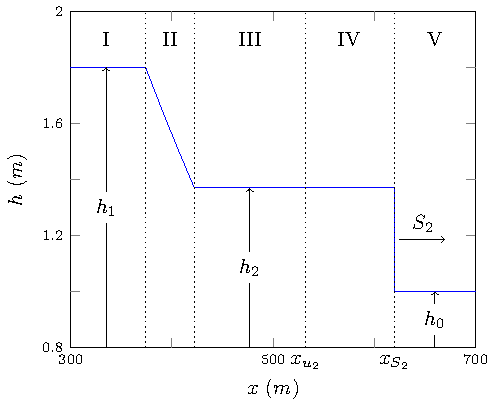
\includegraphics[width=0.5\textwidth]{pics/explainers/SWWEana.pdf}
	\caption{Analytic solution at $t=30s$ of the shallow water wave equations for the dam-break problem with $h_0 = 1m$, $h_1=1.8m$ and $x_0=100m$.}
	\label{fig:SWWEanadiagram}
\end{figure}

\begin{figure}
	\centering
	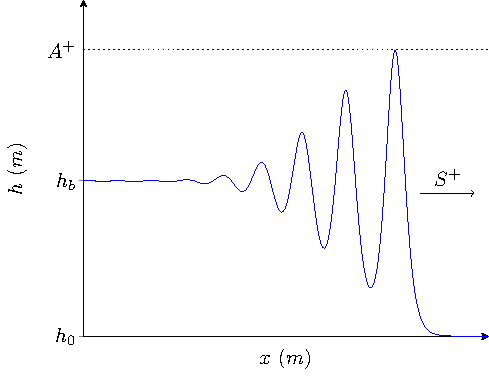
\includegraphics[width=0.5\textwidth]{pics/explainers/SERREex.pdf}
	\caption{Demonstration of quantities obtained by Whitham modulation for undular bores of the Serre equations.}
	\label{fig:Serreanadiagram}
\end{figure}


\subsection{Shallow Water Wave Equation Analytic Solution}
\citet{Hank-etal-2010-2034} and \citet{Mitsotakis-etal-2014} demonstrated that the analytic solution of the shallow water wave equations for the dam-break problem captures the mean behaviour of their numerical results for the Serre equations. In section \ref{section:NumRes} the validity of this comparison is assessed and so the relevant background required for it is presented here.

For the discontinuous dam-break problem the shallow water wave equations, which are the Serre equations with dispersive terms neglected, can be solved analytically. The analytic solution of the shallow water wave equations has been used as a comparative tool against numerical results in the literature \cite{Hank-etal-2010-2034,Mitsotakis-etal-2014} as they appear to capture the mean behaviour of the numerical solutions. 

An example of the analytic solution of the shallow water wave equations for the dam-break problem is presented in Figure \ref{fig:SWWEanadiagram} at $t=30s$. Region I is the undisturbed water upstream of the dam-break at constant height ($h_1$) and velocity ($0m/s$) and region II is the rarefaction fan connecting regions I and III. Regions III and IV are the constant height ($h_2$) and constant velocity ($u_2$) state which are separated by $x_{u_2} = x_0 + u_2t$ and region V is the undisturbed water downstream at constant height ($h_0$) and velocity ($0m/s$) separated from region IV by a shock which travels at velocity $S_2$. Expressions for the unknown quantities $h_2$, $u_2$ and $S_2$ in terms of $h_0$ and $h_1$ were given by \citet{Wu-etal-1999-1210}
\begin{linenomath*}
\begin{subequations}
\begin{gather}
h_2 = \frac{h_0}{2} \left(\sqrt{1 + 8 \left(\frac{2h_2}{h_2 - h_0}\frac{\sqrt{gh_1} - \sqrt{gh_2}}{\sqrt{gh_0}}\right)^2} - 1\right),
\end{gather}
	\begin{gather}
	u_2 = 2\left(\sqrt{gh_1} - \sqrt{gh_2}\right)
	\end{gather}
and
	\begin{gather}
	S_2 = \frac{h_2 u_2}{h_2 - h_0}.
	\end{gather}
\label{eq:WuSWWE}	
\end{subequations}
\end{linenomath*}
Applying \eqref{eq:WuSWWE} to our dam-break problem heights results in $h_2 = 1.36898m$ , $u_2 = 1.074975$ $m/s$ and $S_2 = 3.98835$ $m/s$ which are demonstrated in Figure \ref{fig:SWWEanadiagram}.


\section{Numerical Methods}
\label{sec:nummeth}
%where methods come from
%grid and cells definition
Five numerical schemes are used to solve the Serre equations. The first ($\mathcal{V}_1$), second ($\mathcal{V}_2$) and third-order ($\mathcal{V}_3$) methods of \cite{Zoppou-etal-2017}, the method of \citet{El-etal-2006} ($\mathcal{E}$) and a second-order finite difference method ($\mathcal{G}$).

The $\mathcal{V}_i$ methods are stable under the CFL condition \cite{Harten-etal-1983-357} and have demonstrated the appropriate order of convergence for smooth problems \cite{Zoppou-etal-2017}. Furthermore, $\mathcal{V}_2$ and $\mathcal{V}_3$ have been validated against experimental data containing steep gradients \cite{Zoppou-etal-2017}. The two methods $\mathcal{G}$ and $\mathcal{E}$ were found to be stable under the CFL condition as well, and for completeness these methods are presented in the Appendix to allow for replication.

Generally we find that $\mathcal{V}_1$ is the worst performing of these methods due to its diffusivity \cite{Zoppou-etal-2017}. Of the high-order methods $\mathcal{E}$ is the worst performing, introducing dispersive errors. The methods $\mathcal{V}_2$ and $\mathcal{V}_3$ produce very similar numerical solutions \cite{Zoppou-etal-2017}, while the numerical solutions of $\mathcal{G}$ are also close to them.


%--------------------------------------------------------------------------------
\section{Numerical Results}
\label{section:NumRes}
%--------------------------------------------------------------------------------
We begin by looking into the effect of the initial steepness of the smoothed dam-break problem for different $\alpha$ values by observing what happens as $\Delta x \rightarrow 0$ and our numerical solutions better approximate the true solution of the Serre equations. We then investigate numerical results for long time scales and how the shallow water wave equations analytic solution compare to our numerical solutions. 

All numerical methods used $\Delta t = 0.01 \Delta x$ which is smaller than required by the CFL condition \cite{Harten-etal-1983-357} which ensures stability of our schemes. The time step $\Delta t$ was chosen to be smaller than necessary because for a final time of $t=30s$ making $\Delta t$ small suppresses errors without excessively increasing the run-time of the experiments. The method $\mathcal{V}_2$ requires an input parameter to its slope limiter and this was chosen to be $\theta = 1.2$ \cite{Zoppou-etal-2017}. All of the numerical methods presented use Dirichlet boundary conditions with $u = 0m/s$ at both boundaries and $h =1.8m$ on the left and $h =1m$ on the right.

\subsection{Observed Structures of the Numerical Solutions}
We observe that there are four different structures as $\Delta x \rightarrow 0$ depending on the $\alpha$ and the numerical method. They are the non-oscillatory structure, the flat structure, the node structure and the growth structure. An example of each of these structures is in Figure \ref{fig:allstructs} for $\mathcal{V}_3$'s numerical solutions to various smoothed dam-break problems. 

\begin{figure}
	\centering
	\begin{subfigure}{0.5\textwidth}
		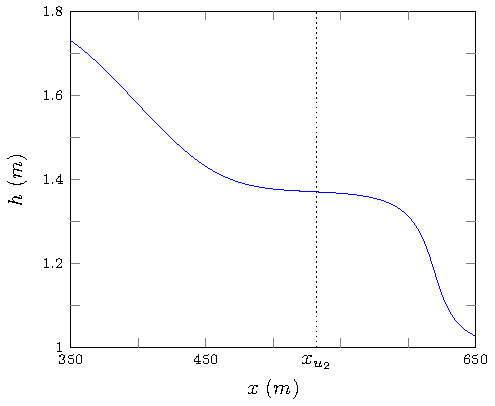
\includegraphics[width=\textwidth]{pics/results/SDB/structs/non.pdf}
		\subcaption*{\hspace{10 mm}Non-oscillatory structure  ($\alpha = 40m$)}
	\end{subfigure}%
	\begin{subfigure}{0.5\textwidth}
		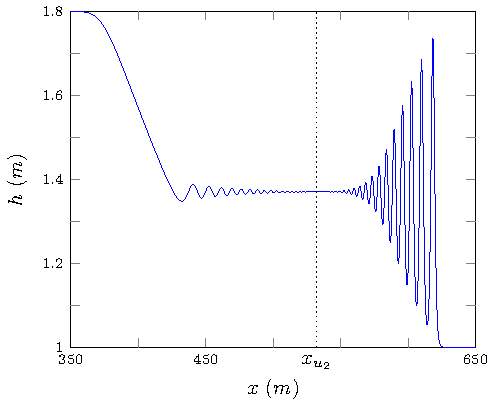
\includegraphics[width=\textwidth]{pics/results/SDB/structs/flat.pdf}
		\subcaption*{\hspace{10 mm} Flat structure ($\alpha = 2m$)}
	\end{subfigure}
	\begin{subfigure}{0.5\textwidth}
		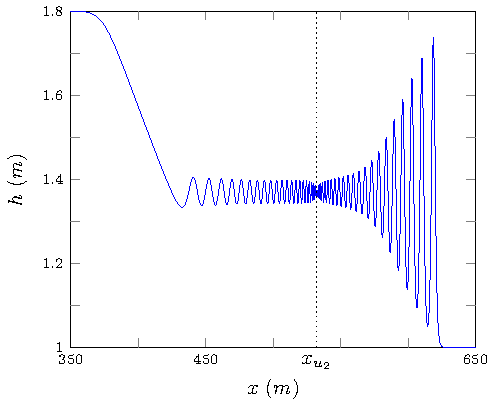
\includegraphics[width=\textwidth]{pics/results/SDB/structs/node.pdf}
		\subcaption*{\hspace{10 mm}Node structure ($\alpha = 0.4m$)}
	\end{subfigure}%
	\begin{subfigure}{0.5\textwidth}
		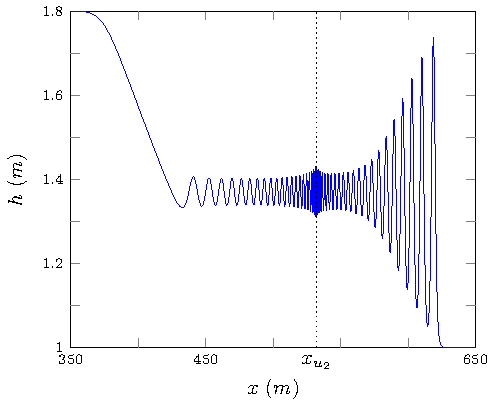
\includegraphics[width=\textwidth]{pics/results/SDB/structs/growth.pdf}
		\subcaption*{\hspace{10 mm}Growth structure ($\alpha = 0.1m$)}
	\end{subfigure}	
	\caption{Numerical results of $\mathcal{V}_3$ with $\Delta x = 10/2^{11}m$ ({\color{blue} \solidrule}) at $t= 30s$ for various smooth dam-break problems demonstrating the different observed structures.}
	\label{fig:allstructs}
\end{figure}

The four structures are identified by the nature of the numerical solutions in regions III and IV when $\Delta x$ is small and they correspond to different structures in the numerical solutions presented in the literature. From Figure \ref{fig:allstructs} it can be seen that as $\alpha$ is decreased, steepening the initial conditions the numerical solutions demonstrate an increase in the size and number of oscillations particularly around $x_{u_2}$. 

For the non-oscillatory and flat structures there is excellent agreement between all higher-order numerical methods at our highest resolution $\Delta x = 10/2^{11}m$. An illustration of this agreement is given in Figure \ref{fig:allmodels2struct} for the flat structure which is the most difficult to resolve of the two structures. Since the first-order scheme is diffusive \cite{Zoppou-etal-2017} we find that although it's highest resolution numerical solution has the same behaviour as the other methods it damps the oscillations.

\begin{figure}
	\centering
	\begin{subfigure}{0.5\textwidth}
		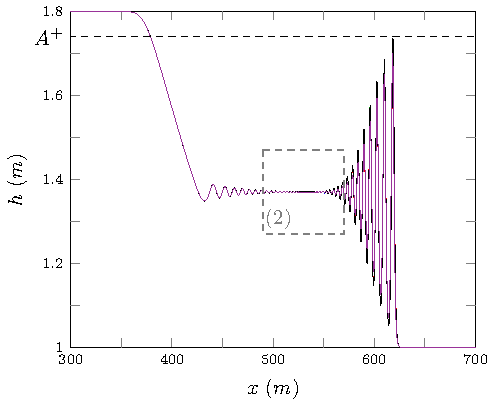
\includegraphics[width=\textwidth]{pics/results/SDB/numsols/modelcompalpha6dx11/1.pdf}
	\end{subfigure}%
	\begin{subfigure}{0.5\textwidth}
		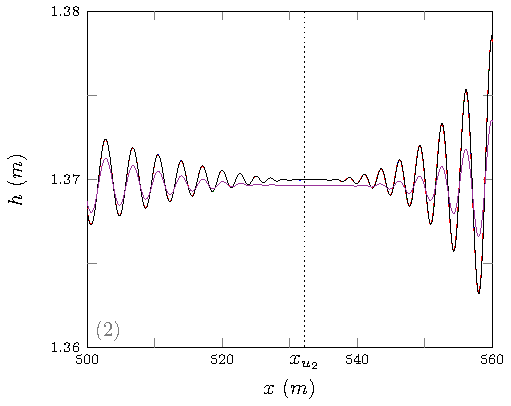
\includegraphics[width=\textwidth]{pics/results/SDB/numsols/modelcompalpha6dx11/2.pdf}
	\end{subfigure}
	
	\caption{Numerical solutions $\mathcal{G}$ ({\color{blue} \solidrule}), $\mathcal{E}$ ({\color{red} \solidrule}), $\mathcal{V}_3$ ({\color{green!60!black} \solidrule}), $\mathcal{V}_2$ ({\color{black} \solidrule}) and $\mathcal{V}_1$ ({\color{violet!60!white} \solidrule}) with $\Delta x = 10/2^{11}m$ at $t= 30s$ for the smooth dam-break problem with $\alpha =2m$.}
	\label{fig:allmodels2struct}
\end{figure}

\subsubsection{Non-oscillatory Structure}
The first structure is the non-oscillatory structure it is the result of a large $\alpha$. When $\alpha$ is large for the smoothed dam-break problem the fluid to the left of $x_0$ flows to fill the right side, but due to the large $\alpha$ the front of this flow is not steep enough to generate undulations over short time spans. Eventually the front of this flow steepens due to non-linearity and undulations develop there.

This structure is not present in the literature as no authors chose large enough $\alpha$. An example of this structure can be seen in Figure \ref{fig:o3a1dxlimnonexp} for $\alpha = 40m$ using $\mathcal{V}_3$. Because this is a very smooth problem we observe that all numerical results are visually identical for all $\Delta x < 10 / 2^4m$.

From Table \ref{tab:L1C1} it can be seen that not only have these solutions converged visually but the $L_1$ measures demonstrate that we have reached convergence to round-off error by $\Delta x = 10 / 2^8m$ after which the relative difference between numerical solutions plateau. 

Table \ref{tab:L1C1} also demonstrates that the error in conservation of the numerical solutions are at round-off error for $h$ and $\mathcal{H}$. $C^{uh}_1$ is the worst performing of the measures because the smoothed dam-break has such a large $\alpha$ that $h(0m) \neq 1.8m$ and $h(1000m) \neq 1m$ causing unequal fluxes in momentum at the boundaries.  

Because the initial conditions are not steep enough an undular bore has not developed by $t=30s$ thus the Whitham modulation results for leading wave amplitude do not apply.

The convergence and conservation of numerical solutions as $\Delta x \rightarrow 0$ together with the agreement of different numerical methods demonstrates that the numerical result in Figure \ref{fig:o3a1dxlimnonexp} and its non-oscillatory structure is an accurate representation of the solutions of the Serre equations when $\alpha$ is sufficiently large and in particular $\alpha = 40m$. 
\begin{figure}
	\centering
	\begin{subfigure}{0.5\textwidth}
		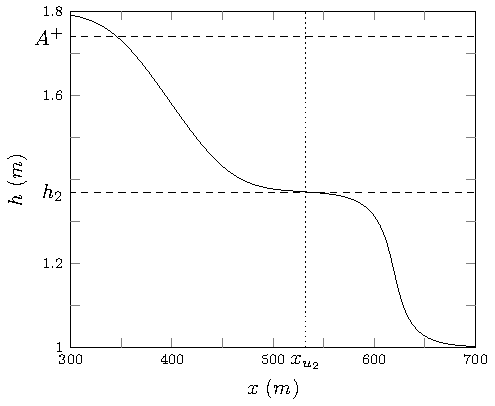
\includegraphics[width=\textwidth]{pics/results/SDB/numsols/alpha0.025/1-figure0.pdf}
	\end{subfigure}%
	
	\caption{Numerical results of $\mathcal{V}_3$  at $t= 30s$ for smooth dam-break problem with $\alpha = 40m$ for $\Delta x = 10/2^{10}m$ ({\color{blue} \solidrule}), $10/2^8m$ ({\color{red} \solidrule}), $10/2^6m$ ({\color{green!60!black} \solidrule}) and $10/2^{4}m$ ({\color{black} \solidrule}).}
	\label{fig:o3a1dxlimnonexp}
\end{figure}

\begin{table}
\begin {tabular}{c c c c c c c}%
$\alpha$& $\Delta x$&$C_1^{h}$&$C_1^{uh}$&$C_1^{\mathcal {H}}$&$L_1^{h}$&$L_1^{u}$\\%
\hline\hline\\
$40$ &$10/2^{4}$& 1\pgfutilensuremath {2\cdot 10^{-11}}&\pgfutilensuremath {1.77\cdot 10^{-6}}&\pgfutilensuremath {1.23\cdot 10^{-8}}&\pgfutilensuremath {1.74\cdot 10^{-7}}&\pgfutilensuremath {2.90\cdot 10^{-6}}\\%
$40$ &$10/2^{6}$& \pgfutilensuremath {1.07\cdot 10^{-11}}&\pgfutilensuremath {1.50\cdot 10^{-6}}&\pgfutilensuremath {1.49\cdot 10^{-10}}&\pgfutilensuremath {2.57\cdot 10^{-9}}&\pgfutilensuremath {4.19\cdot 10^{-8}}\\%
$40$ &$10/2^{8}$& \pgfutilensuremath {8.77\cdot 10^{-13}}&\pgfutilensuremath {5.49\cdot 10^{-7}}&\pgfutilensuremath {3.77\cdot 10^{-13}}&\pgfutilensuremath {6.08\cdot 10^{-11}}&\pgfutilensuremath {5.28\cdot 10^{-10}}\\%
$40$ &$10/2^{10}$& \pgfutilensuremath {1.77\cdot 10^{-11}}&\pgfutilensuremath {2.21\cdot 10^{-8}}&\pgfutilensuremath {3.56\cdot 10^{-11}}&\pgfutilensuremath {2.54\cdot 10^{-11}}&\pgfutilensuremath {6.49\cdot 10^{-11}}\\%
\hline \\
$2$ &$10/2^{4}$&\pgfutilensuremath {4.9\cdot 10^{-14}}&\pgfutilensuremath {5.10\cdot 10^{-3}}&\pgfutilensuremath {8.69\cdot 10^{-4}}&\pgfutilensuremath {5.02\cdot 10^{-3}}&\pgfutilensuremath {6.77\cdot 10^{-2}}\\%
$2$ &$10/2^{6}$&\pgfutilensuremath {2.51\cdot 10^{-13}}&\pgfutilensuremath {2.18\cdot 10^{-4}}&\pgfutilensuremath {6.58\cdot 10^{-5}}&\pgfutilensuremath {4.14\cdot 10^{-4}}&\pgfutilensuremath {5.20\cdot 10^{-3}}\\%
$2$ &$10/2^{8}$&\pgfutilensuremath {9.81\cdot 10^{-13}}&\pgfutilensuremath {7.72\cdot 10^{-7}}&\pgfutilensuremath {5.01\cdot 10^{-7}}&\pgfutilensuremath {6.00\cdot 10^{-6}}&\pgfutilensuremath {7.59\cdot 10^{-5}}\\%
$2$ &$10/2^{10}$&\pgfutilensuremath {3.95\cdot 10^{-12}}&\pgfutilensuremath {5.56\cdot 10^{-9}}&\pgfutilensuremath {6.13\cdot 10^{-9}}&\pgfutilensuremath {1.76\cdot 10^{-7}}&\pgfutilensuremath {2.33\cdot 10^{-6}}\\%
\hline \\
$0.4$ &$10/2^{4}$&\pgfutilensuremath {9\cdot 10^{-14}}&\pgfutilensuremath {4.82\cdot 10^{-3}}&\pgfutilensuremath {1.02\cdot 10^{-3}}&\pgfutilensuremath {6.79\cdot 10^{-3}} $\dagger$&\pgfutilensuremath {9.93\cdot 10^{-2}} $\dagger$\\%
$0.4$ &$10/2^{6}$&\pgfutilensuremath {2.4\cdot 10^{-13}}&\pgfutilensuremath {2.41\cdot 10^{-4}}&\pgfutilensuremath {1.11\cdot 10^{-4}}&\pgfutilensuremath {8.89\cdot 10^{-4}} $\dagger$&\pgfutilensuremath {1.13\cdot 10^{-2}} $\dagger$\\%
$0.4$ &$10/2^{8}$&\pgfutilensuremath {9.68\cdot 10^{-13}}&\pgfutilensuremath {7.57\cdot 10^{-7}}&\pgfutilensuremath {2.25\cdot 10^{-6}}&\pgfutilensuremath {1.53\cdot 10^{-5}} $\dagger$&\pgfutilensuremath {1.91\cdot 10^{-4}} $\dagger$\\%
$0.4$ &$10/2^{10}$&\pgfutilensuremath {3.91\cdot 10^{-12}}&\pgfutilensuremath {4.95\cdot 10^{-9}}&\pgfutilensuremath {2.01\cdot 10^{-8}}&\pgfutilensuremath {3.61\cdot 10^{-7}} $\dagger$&\pgfutilensuremath {5.00\cdot 10^{-6}} $\dagger$\\%
\hline \\
$0.1$ &$10/2^{4}$&\pgfutilensuremath {7.6\cdot 10^{-14}}&\pgfutilensuremath {4.82\cdot 10^{-3}}&\pgfutilensuremath {1.06\cdot 10^{-3}}&\pgfutilensuremath {7.04\cdot 10^{-3}} $\dagger$&\pgfutilensuremath {1.02\cdot 10^{-1}} $\dagger$\\%
$0.1$ &$10/2^{6}$&\pgfutilensuremath {2.4\cdot 10^{-13}}&\pgfutilensuremath {2.39\cdot 10^{-4}}&\pgfutilensuremath {1.44\cdot 10^{-4}}&\pgfutilensuremath {1.02\cdot 10^{-3}} $\dagger$&\pgfutilensuremath {1.28\cdot 10^{-2}} $\dagger$\\%
$0.1$ &$10/2^{8}$&\pgfutilensuremath {9.79\cdot 10^{-13}}&\pgfutilensuremath {2.21\cdot 10^{-7}}&\pgfutilensuremath {1.20\cdot 10^{-5}}&\pgfutilensuremath {2.86\cdot 10^{-5}} $\dagger$&\pgfutilensuremath {3.46\cdot 10^{-4}} $\dagger$\\%
$0.1$ &$10/2^{10}$&\pgfutilensuremath {3.92\cdot 10^{-12}}&\pgfutilensuremath {4.46\cdot 10^{-8}}&\pgfutilensuremath {7.61\cdot 10^{-7}}&\pgfutilensuremath {4.99\cdot 10^{-7}} $\dagger$&\pgfutilensuremath {6.40\cdot 10^{-6}} $\dagger$\\%
\end {tabular}%
\caption{All errors in conservation $C^{q}_1$ for the conserved quantities and relative distances $L^{q}_1$ of the primitive variables for numerical solutions of $\mathcal{V}_3$. $L^{q}_1$ uses the numerical solution with $\Delta x = 10/2^{11}m$ as the high resolution basis of comparison and $\dagger$ indicates the omission of the interval [$520m$, $540m$] from the comparison.}
\label{tab:L1C1}
\end{table}

\subsubsection{Flat Structure}
The second structure will be referred to as the flat structure due to the presence of a constant height around $x_{u_2}$, this is the most common structure observed in the literature \cite{Hank-etal-2010-2034,Mitsotakis-etal-2014,Mitsotakis-etal-2017}. It is generated as are the rest of the structures when the initial conditions are steep enough such that the bore that develops has undulations. This structure consists of oscillations in regions III and IV which are separated by a constant height state around $x_{u_2}$. An example of the structure can be seen in the numerical solutions presented in Figure \ref{fig:o3a6dxlimflatexp} when $\alpha = 2m$.

As $\Delta x$ decreases the numerical solutions converge so that by $\Delta x = 10 / 2^8m$ the solutions for higher $\Delta x$ are visually identical. Table \ref{tab:L1C1} demonstrates that although we have convergence visually the $L_1$ measures are still decreasing and haven't plateaued. Likewise the $C_1$ are still decreasing and have only reached round-off error for $h$, although our numerical solutions are close to one another and exhibit good conservation. This indicates that to precisely resolve the numerical solutions for $\mathcal{V}_3$ of this smoothed dam-break problem down to round-off error would require an even lower $\Delta x$.

Figures \ref {fig:o3a6dxlimflatexp} and \ref{fig:allmodels2struct} demonstrate good agreement between the numerical solutions and $A^+$ derived from the Whitham modulation of \citet{El-etal-2006}.

The convergence of our numerical solutions as $\Delta x \rightarrow 0$ of $\mathcal{V}_3$ both in Figure \ref {fig:o3a6dxlimflatexp} and Table \ref{tab:L1C1}, the agreement of all the models in Figure \ref{fig:allmodels2struct} with $\Delta x=10/2^{11}m$ and agreement of the numerical solutions and $A^+$ demonstrates that while our solutions have not converged down to round-off error our numerical solutions are accurate approximate solutions of the Serre equations for the smoothed dam-break problem with $\alpha = 0.5m$.


These numerical solutions compare well with those of \citet{Mitsotakis-etal-2014} who use the same $\alpha$ but different $h_0$ and $h_1$ and resolve the same behaviour. We found that we resolved this structure for all methods at $\Delta x = 10/2^{11}m$ for the smoothed dam-break with $\alpha$'s as low as $1m$. This is the same behaviour that is present in the numerical solutions of \citet{Mitsotakis-etal-2017} who use $\alpha=1m$ but different heights. Therefore \citet{Mitsotakis-etal-2014} and \citet{Mitsotakis-etal-2017} only observe the flat scenario in their numerical results due to their choice of $\alpha$ for the smoothed dam-break problem. 

The first-order $\mathcal{V}_1$ is diffusive \cite{Zoppou-etal-2017} and damps oscillations that are present in higher-order methods numerical results as in Figure \ref{fig:allmodels2struct}. We find that for any $\alpha \le 4m$ and the discontinuous dam-break problem our numerical solutions of $\mathcal{V}_1$ at $t=30s$ with $\Delta x = 10/2 ^{11}m$ can only resolve the flat scenario which can be seen in Figure \ref{fig:o1highdchigha} for $\alpha = 0.001m$. Therefore \citet{Hank-etal-2010-2034} using $\mathcal{V}_1$ with their chosen $\Delta x$ and $\Delta t$ which are larger than our $\Delta x$ and $\Delta t$ could only resolve the flat structure. 

\begin{figure}
	\begin{subfigure}{\textwidth}
		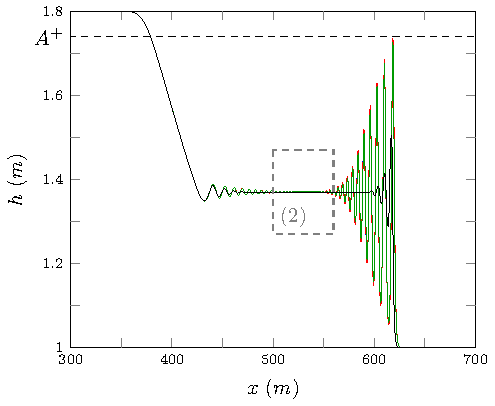
\includegraphics[width=0.5\textwidth]{pics/results/SDB/numsols/alpha0.5/1-figure0.pdf}
		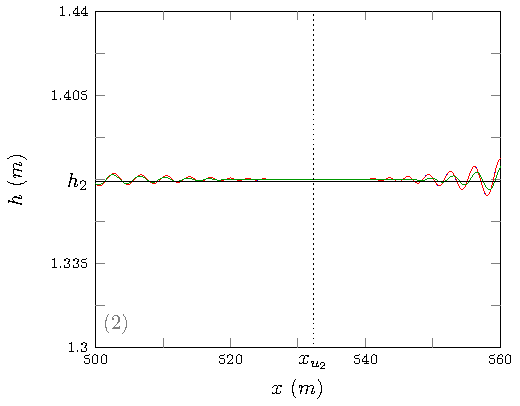
\includegraphics[width=0.525\textwidth]{pics/results/SDB/numsols/alpha0.5/2-figure0.pdf}
	\end{subfigure}
\caption{Numerical results of $\mathcal{V}_3$  at $t= 30s$ for the smooth dam-break problem with $\alpha = 2m$ for $\Delta x = 10/2^{10}m$ ({\color{blue} \solidrule}), $10/2^8m$ ({\color{red} \solidrule}), $10/2^6m$ ({\color{green!60!black} \solidrule}) and $10/2^{4}m$ ({\color{black} \solidrule}).}
\label{fig:o3a6dxlimflatexp}
\end{figure}

\begin{figure}
	\centering
	\begin{subfigure}{\textwidth}
		\centering
		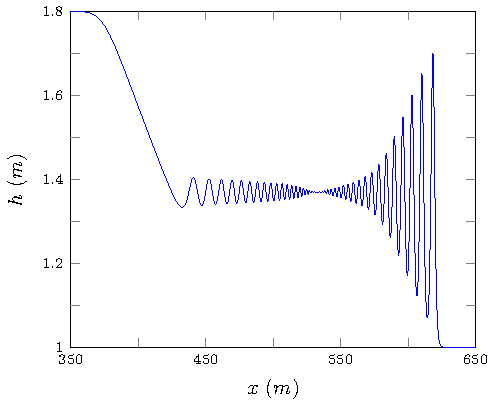
\includegraphics[width=0.5\textwidth]{pics/results/SDB/structs/o1flathigh.pdf}
	\end{subfigure}
	\caption{Numerical solution of $\mathcal{V}_1$  at $t= 30s$ for the smooth dam-break problem with $\alpha = 0.001m$ for $\Delta x = 10/2^{11}m$ ({\color{blue} \solidrule}).}
	\label{fig:o1highdchigha}
\end{figure}


\subsubsection{Node Structure}
The third structure will be referred to as the node structure and it is was observed by \citet{El-etal-2006}. The node structures main feature is that the oscillations in region III and IV decay and appear to meet at $x_{u_2}$ as can be seen in Figure \ref{fig:o3a9dxlimcdexp} when $\alpha = 0.4m$.

Figure \ref{fig:o3a9dxlimcdexp} demonstrates that our numerical solutions have not converged, however this is only in the area around $x_{u_2}$. Due to the large difference in numerical solutions around $x_{u_2}$ the $L_1$ measure over the area around $x_{u_2}$ would not be insightful, however by omitting this region we can gain some knowledge about how well our solutions agree away from $x_{u_2}$. This was performed for the  relevant $L_1$ measures in Table \ref{tab:L1C1} by omitting the interval [$520m$, $540m$]. These modified $L_1$ measures demonstrate that while our numerical results have visually converged away from $x_{u_2}$ they have not fully converged down to round-off error under the $L_1$ measure although they are close to one another away from $x_{u_2}$. 

Table \ref{tab:L1C1} demonstrates that the $C_1$ measures are decreasing as well and have only reached round-off error for $h$. Therefore to resolve the converged numerical solution of this particular smoothed dam-break problem down would require even lower $\Delta x$ values.  

There is a good agreement across different numerical methods for $\Delta x = 10/2^{11}m$ as can be seen in Figure \ref{fig:o3a9allmodels}. In particular all the higher-order methods exhibit the same behaviour and most only disagree in a very small region around $x_{u_2}$, although we observe that $\mathcal{E}$ has not converged as well to the numerical solutions of the other methods. 

Figures \ref{fig:o3a9dxlimcdexp} and \ref{fig:o3a9allmodels} demonstrate good agreement between the numerical solutions and $A^+$ derived from Whitham modulation across different methods and different $\Delta x$.

The behaviour of $\mathcal{V}_3$'s solutions as $\Delta x \rightarrow 0$, the agreement of different numerical methods when $\Delta x = 10 / 2^{11}m$  and the agreement of our numerical solutions with $A^+$ demonstrates that while our numerical solutions have not completely visually converged they are an accurate representation of the solutions of the Serre equations for the smoothed dam-break problem with $\alpha = 0.4m$. In particular for $\alpha = 0.4m$ the node structure should be observed in numerical solutions of the Serre equations.

These numerical solutions support the findings of \citet{El-etal-2006} who also use some smoothing \cite{El-Hoefer-2016-11} but do not report what smoothing was performed. Using their method $\mathcal{E}$ and similar $\Delta x$ to \citet{El-etal-2006} we are able to resolve the growth behaviour for smaller $\alpha$'s, indicating that the smoothing performed by \citet{El-etal-2006} limited their observed behaviour to just the node structure. 

\begin{figure}
\centering
\begin{subfigure}{\textwidth}
	\centering
	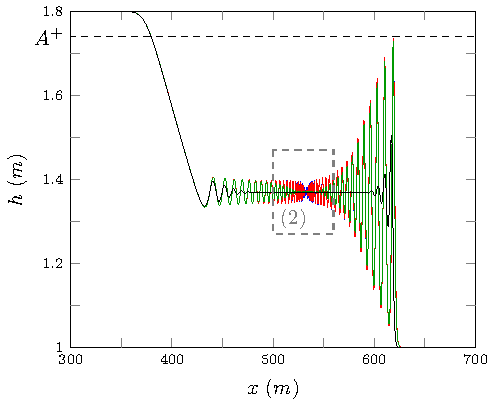
\includegraphics[width=0.65\textwidth]{pics/results/SDB/numsols/alpha2.5/1-figure0.pdf}
\end{subfigure}
\begin{subfigure}{\textwidth}
	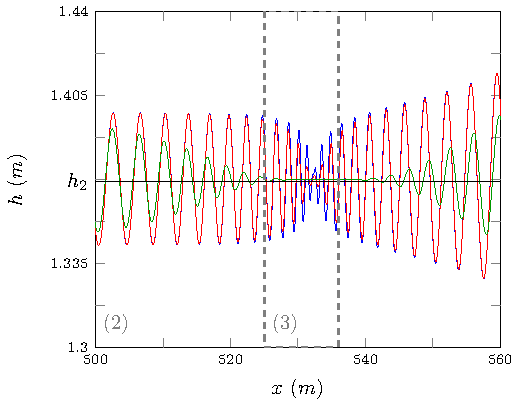
\includegraphics[width=0.5\textwidth]{pics/results/SDB/numsols/alpha2.5/2-figure0.pdf}
	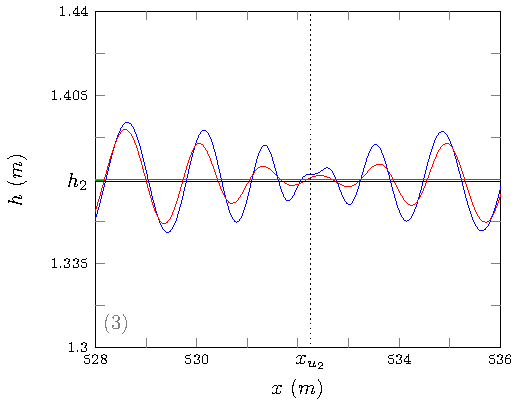
\includegraphics[width=0.5\textwidth]{pics/results/SDB/numsols/alpha2.5/3-figure0.pdf}
\end{subfigure}
\caption{Numerical solution of $\mathcal{V}_3$  at $t= 30s$ for the smooth dam-break problem with $\alpha = 0.4m$ for $\Delta x = 10/2^{10}m$ ({\color{blue} \solidrule}), $10/2^8m$ ({\color{red} \solidrule}), $10/2^6m$ ({\color{green!60!black} \solidrule}) and $10/2^{4}m$ ({\color{black} \solidrule}).}
\label{fig:o3a9dxlimcdexp}
\end{figure}

\begin{figure}
	\centering
	\begin{subfigure}{\textwidth}
		\centering
		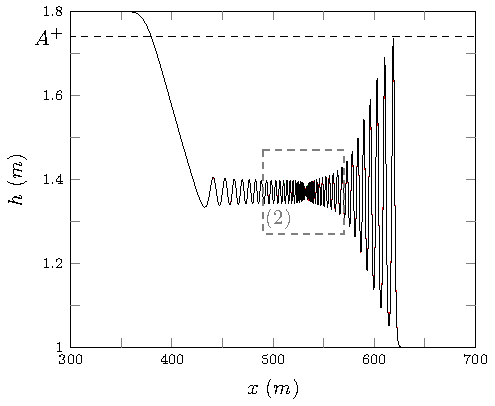
\includegraphics[width=0.65\textwidth]{pics/results/SDB/numsols/modelcompalpha9dx11/1.pdf}
	\end{subfigure}
	\begin{subfigure}{\textwidth}
		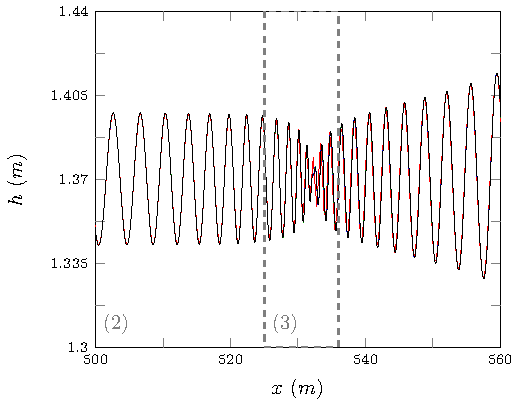
\includegraphics[width=0.5\textwidth]{pics/results/SDB/numsols/modelcompalpha9dx11/2.pdf}
		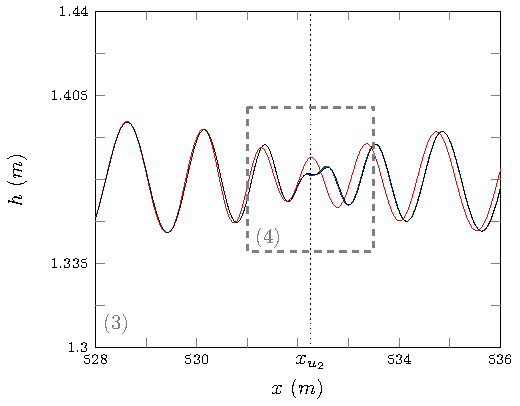
\includegraphics[width=0.5\textwidth]{pics/results/SDB/numsols/modelcompalpha9dx11/4.pdf}
	\end{subfigure}
	\caption{Numerical solution of $\mathcal{G}$ ({\color{blue} \solidrule}), $\mathcal{E}$ ({\color{red} \solidrule}), $\mathcal{V}_3$ ({\color{green!60!black} \solidrule}) and $\mathcal{V}_2$ ({\color{black} \solidrule}) at $t=30s$ with $\Delta x = 10/2^{11}m$ for the smoothed dam-break problem with $\alpha = 0.4m$.}
	\label{fig:o3a9allmodels}
\end{figure}


\subsubsection{Growth Structure}
The fourth structure is the growth structure which has hitherto not been published. It features a growth in the oscillation amplitude around $x_{u_2}$. An example of the growth structure can be seen for $\mathcal{V}_3$'s numerical solutions in Figure \ref{fig:o3a20dxlimcdexp} of the smoothed dam-break problem with $\alpha = 0.1m$. This structure was observed in the numerical solutions of $\mathcal{V}_3$ for $\Delta x = 10/2^{11}m$ at $t=30s$ for $\alpha$'s as low as $0.001m$ and even for the discontinuous dam-break problem.

Figure \ref{fig:o3a20dxlimcdexp} shows that this behaviour can only be observed for $\Delta x = 10 / 2^{10}m$, with poor convergence of the numerical results around $x_{u_2}$. Again our $L_1$ measures in Table \ref{tab:L1C1} omit the interval [$520m$,$540m$] to compare the numerical solutions. This demonstrates that away from $x_{u_2}$ our numerical solutions are quite close to one another but they have not converged to round-off error as $\Delta x \rightarrow 0$. The $C_1$ measures in Table \ref{tab:L1C1} are still decreasing and have only attained round-off error for $h$, although for $uh$ and $\mathcal{H}$ the errors in  conservation are still small. These measures continue the trend in Table \ref{tab:L1C1} where smaller $\alpha$'s and thus steeper initial conditions lead to poorer convergence and conservation because they are more difficult to solve accurately.

Figures \ref{fig:o3a20dxlimcdexp} and \ref{fig:o3a12allmodels} demonstrate good agreement between the numerical solutions and $A^+$ derived from Whitham modulation.

Figure \ref{fig:o3a12allmodels} demonstrates that our numerical solutions for $\Delta x = 10 /2^{11}m$ with the best methods $\mathcal{E}$, $\mathcal{V}_3$ and $\mathcal{V}_2$ disagree for only a few oscillations around $x_{u_2}$. Since both $\mathcal{G}$ and $\mathcal{E}$ are second-order finite difference methods their errors are dispersive meaning that oscillation size and number in their numerical solutions are overestimated, as can be seen for the large dispersive errors of $\mathcal{E}$. All $\mathcal{V}_i$ methods are diffusive and therefore underestimate the size and number of oscillations in their numerical solutions. Therefore the true solution of the Serre equations should be between the dispersive method $\mathcal{G}$ and the diffusive method $\mathcal{V}_3$ which is a growth structure. 

These results indicate that the solutions of the Serre equations to the smoothed dam-break with sufficiently small $\alpha$'s should exhibit a growth structure at $t=30s$, even though we have not precisely resolved all the oscillations in our numerical solutions. 

It was found that decreasing $\alpha$ did increase the amplitude of the oscillations around $x_{u_2}$ but not drastically, for $\mathcal{V}_3$ with $\Delta x= 10/2^{11}m$ and $\alpha = 0.001m$ the oscillations in $h$ were bounded by the interval [$1.28m$,$1.46m$]. Of particular note is that the number of oscillations are the same in Figures \ref{fig:o3a9allmodels} and \ref{fig:o3a12allmodels} for the best methods even though they have different structures.

\begin{figure}
\centering
\begin{subfigure}{\textwidth}
	\centering
	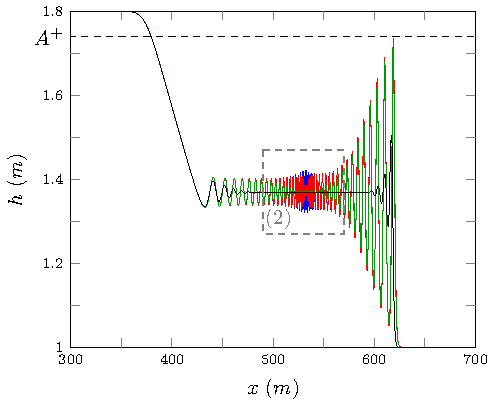
\includegraphics[width=0.65\textwidth]{pics/results/SDB/numsols/alpha10/1-figure0.pdf}
\end{subfigure}
\begin{subfigure}{\textwidth}
	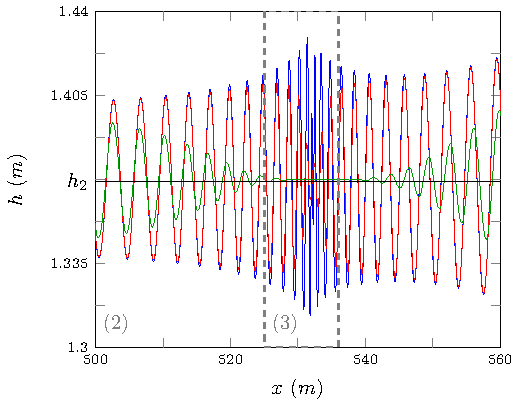
\includegraphics[width=0.5\textwidth]{pics/results/SDB/numsols/alpha10/2-figure0.pdf}
	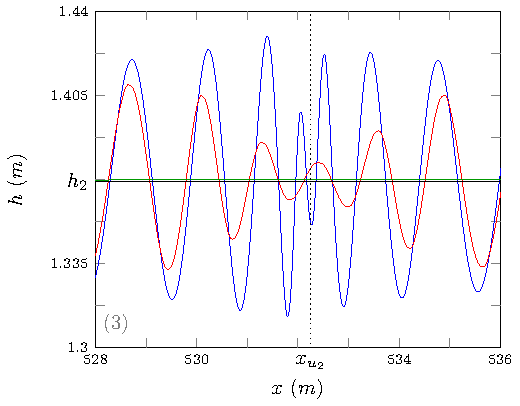
\includegraphics[width=0.5\textwidth]{pics/results/SDB/numsols/alpha10/3-figure0.pdf}
\end{subfigure}
\caption{Numerical solutions of $\mathcal{V}_3$  at $t= 30s$ for the smooth dam-break problem with $\alpha = 0.1m$ for $\Delta x = 10/2^{10}m$ ({\color{blue} \solidrule}), $10/2^8m$ ({\color{red} \solidrule}), $10/2^6m$ ({\color{green!60!black} \solidrule}) and $10/2^{4}m$ ({\color{black} \solidrule}).}
\label{fig:o3a20dxlimcdexp}
\end{figure}

\begin{figure}
	\centering
	\begin{subfigure}{\textwidth}
		\centering
		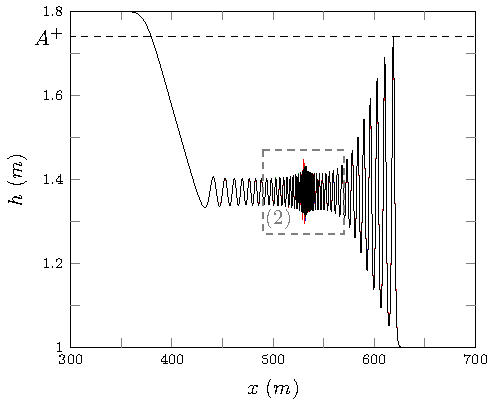
\includegraphics[width=0.65\textwidth]{pics/results/SDB/numsols/modelcompalpha12dx11/1.pdf}
	\end{subfigure}
	\begin{subfigure}{\textwidth}
		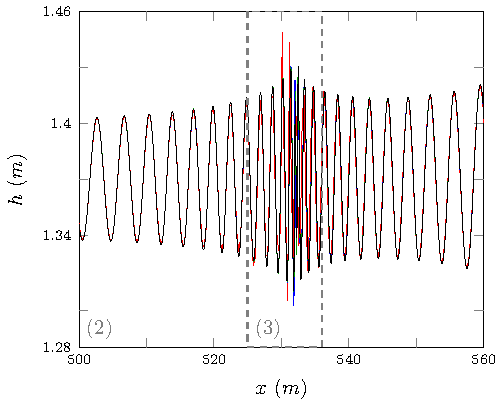
\includegraphics[width=0.5\textwidth]{pics/results/SDB/numsols/modelcompalpha12dx11/2.pdf}
		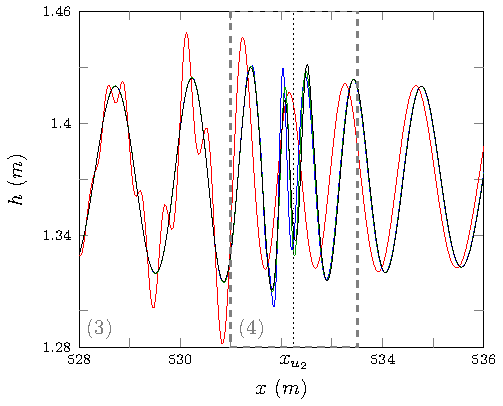
\includegraphics[width=0.5\textwidth]{pics/results/SDB/numsols/modelcompalpha12dx11/4.pdf}
	\end{subfigure}
	\caption{Numerical solutions of $\mathcal{G}$ ({\color{blue} \solidrule}), $\mathcal{E}$ ({\color{red} \solidrule}), $\mathcal{V}_3$ ({\color{green!60!black} \solidrule}) and $\mathcal{V}_2$ ({\color{black} \solidrule}) at $t=30s$ with $\Delta x = 10/2^{11}m$ for the smoothed dam-break problem with $\alpha = 0.1m$.}
	\label{fig:o3a12allmodels}
\end{figure}

\subsection{Shallow water wave equation comparison}
The analytic solutions of shallow water wave equations have been used as a guide for the mean behaviour of the solution of the Serre equations for the dam-break problem in the literature \cite{Hank-etal-2010-2034,Mitsotakis-etal-2014}. 

To assess the applicability of this the mean of our numerical solution of $u$ and $h$ in the interval [$x_{u_2}-50m$,$x_{u_2}+50m$] were calculated for a range of different smoothed dam-break height ratios and compared to their respective approximation from the shallow water wave equations $u_2$ and $h_2$. The results of this can be seen in Figure \ref{fig:ratiotest} for numerical solutions of $\mathcal{V}_3$ where $\Delta x = 10/2^{10}m$ for the smoothed dam-break with $\alpha=0.1m$ at $t=100s$ where $h_0$ is fixed and $h_1$ is varied. It can be seen that although these results are not precise the values $h_2$ and $u_2$ are good approximations to the mean behaviour of the fluid inside the bore for a range of different aspect ratios.
 
\begin{figure}
	\centering
	\begin{subfigure}{0.5\textwidth}
		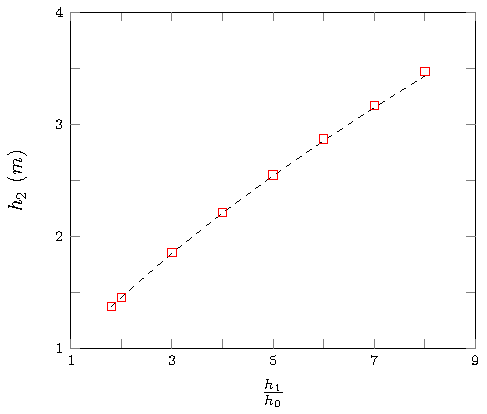
\includegraphics[width=\textwidth]{pics/results/SDB/SWWcomp/meanh.pdf}
		\subcaption*{\hspace{10 mm}h ({\color{red} $\square$}) and $h_2$({\color{black} \dashedrule})}
	\end{subfigure}%
	\begin{subfigure}{0.51\textwidth}
		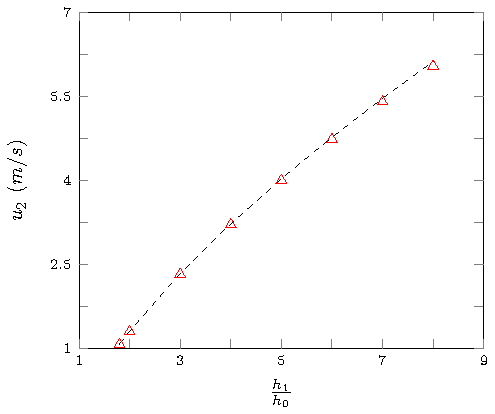
\includegraphics[width=\textwidth]{pics/results/SDB/SWWcomp/meanu.pdf}
		\subcaption*{\hspace{10 mm}u ({\color{red} $\triangle$}) and $u_2$({\color{black} \dashedrule})}
	\end{subfigure}
	\caption{Comparison between mean behaviour of the Serre equations and the values of the analytic solution of the shallow water wave equations that approximate them for a range of different aspect ratios.}
	\label{fig:ratiotest}
\end{figure}

%--------------------------------------------------------------------------------
\section{Conclusions}
\label{section:Conclusions}
%--------------------------------------------------------------------------------
Utilising two finite difference methods of second-order and three finite difference-volume hybrid methods of various orders an investigation into the smoothed dam-break problem with varying steepness was performed. Four different structures of the numerical solutions were uncovered and demonstrated to be valid, the general trend of these structures is that an increase in steepness increases the size and number of oscillations in the solution. This study explains the different structures exhibited by the numerical results in the literature for the solution of the smoothed dam-break problem for Serre equations and uncovers a new result. We find that the analytic solution of the shallow water wave equations for the dam-break problem is a good guide to the mean behaviour of the Serre equations for the smoothed dam-break problem with various aspect ratios.

%more research


%--------------------------------------------------------------------------------
\bibliography{DamBreak}
\bibliographystyle{elsarticle-num-names}
%--------------------------------------------------------------------------------
\appendix{}
\section{}
%--------------------------------------------------------------------------------
The methods $\mathcal{E}$ and $\mathcal{G}$ use the centred second-order finite difference approximation to the conservation of momentum equation \eqref{eq:Serre_momentum} denoted as $\mathcal{G}_u$. For the conservation of mass equation \eqref{eq:Serre_continuity} $\mathcal{E}$ uses the two step Lax-Wendroff method denoted as $\mathcal{E}_h$ while $\mathcal{G}$ uses a centred second-order finite difference approximation denoted as $\mathcal{G}_h$.
\subsection{$\mathcal{G}_u$ for Conservation of Momentum Equation}
The finite difference approximation to \eqref{eq:Serre_momentum} on our grid is
\begin{linenomath*}
	\begin{gather}
	h^{n}_iu^{n+1}_i - \left(h^{n}_i\right)^2 \left(\frac{u^{n+1}_{i+1} -u^{n+1}_{i-1} }{2 \Delta x}\right) - \frac{\left(h^{n}_i\right)^3}{3}\left(\frac{u^{n+1}_{i+1} - 2u^{n+1}_{i} + u^{n+1}_{i-1} }{\Delta x^2}\right) = - Y^n_i
	\label{eq:expandedutdisc3}
	\end{gather}
\end{linenomath*}
and
\begin{linenomath*}
	\begin{gather*}
	Y_i^n = 2\Delta tX_i^{n} - h_i^{n}u_i^{n-1} + \left(h_i^{n}\right)^2\left(\frac{u^{n-1}_{i+1} -u^{n-1}_{i-1} }{2 \Delta x}\right) + \frac{\left(h_i^{n}\right)^3}{3}\left(\frac{u^{n-1}_{i+1} - 2u^{n-1}_{i} + u^{n-1}_{i-1} }{\Delta x^2}\right).
	\label{eq:expandfactor Xp}
	\end{gather*}
\end{linenomath*}
 Equation \eqref{eq:expandedutdisc3} can be rearranged into an explicit update scheme $\mathcal{G}_u$ for $u$ given its current and previous values, so that
\begin{linenomath*}
	\begin{gather}
	\left[\begin{array}{c}
	u^{n+1}_0 \\
	\vdots \\
	u^{n+1}_m \end{array}\right]
	= A^{-1} \left[\begin{array}{c}
	-Y^n_0 \\
	\vdots \\
	-Y^n_m \end{array}\right] =: \mathcal{G}_u\left(\boldsymbol{u}^n,\boldsymbol{h}^n, \boldsymbol{u}^{n-1}, \Delta x, \Delta t \right)
	\label{eq:FDcentforu}
	\end{gather}
\end{linenomath*}
where $A$ is a tri-diagonal matrix.

\subsection{Numerical Methods for Conservation of Mass Equation}
\label{section:}
The two step Lax-Wendroff update $\mathcal{E}_h$ for $h$ is
\begin{linenomath*}
	\begin{gather*}
	h^{n + 1/2}_{i+ 1/2} = \frac{1}{2}\left(h^{n}_{i+1} + h^{n}_i\right) - \frac{\Delta t}{2\Delta x}\left(u^n_{i+1}h^n_{i+1} - h^n_{i}u^n_{i}\right),
	\end{gather*}
	\begin{gather*}
	h^{n + 1/2}_{i- 1/2} = \frac{1}{2}\left(h^{n}_{i} + h^{n}_{i-1}\right) - \frac{\Delta t}{2\Delta x}\left(u^n_{i}h^n_{i} - h^n_{i-1}u^n_{i-1}\right)
	\end{gather*}
	and
	\begin{gather*}
	h^{n+1}_i = h^{n}_i - \frac{\Delta t}{\Delta x}\left(u^{n + 1/2}_{i+ 1/2}h^{n + 1/2}_{i+ 1/2} - u^{n + 1/2}_{i- 1/2}h^{n + 1/2}_{i- 1/2}\right).
	\label{eq:LW4h}
	\end{gather*}
\end{linenomath*}
The quantities $u^{n + 1/2}_{i \pm 1/2}$ are calculated using $u^{n+1}$ obtained by applying $\mathcal{G}_u$ \eqref{eq:FDcentforu} to $u^n$ then linearly interpolating in space and time to give
\begin{linenomath*}
	\begin{gather*}
	u^{n + 1/2}_{i+ 1/2} = \frac{u^{n+1}_{i+1} + u^{n}_{i+1} + u^{n+1}_{i} + u^{n}_{i} }{4}
	\end{gather*}
	and
	\begin{gather*}
	u^{n + 1/2}_{i- 1/2} = \frac{u^{n+1}_{i} + u^{n}_{i} + u^{n+1}_{i-1}+ u^{n}_{i-1} }{4}.
	\end{gather*}
\end{linenomath*}
Thus we have the following update scheme $\mathcal{E}_h$ for \eqref{eq:Serre_continuity}
\begin{linenomath*}
	\begin{gather}
	\boldsymbol{h}^{n+1} = \mathcal{E}_h\left(\boldsymbol{u}^n,\boldsymbol{h}^n,\boldsymbol{u}^{n+1}, \Delta x, \Delta t \right). 
	\label{eq:LWupdateh}
	\end{gather}
\end{linenomath*}


The second order centered finite difference approximation to the conservation of mass equation \eqref{eq:Serre_continuity} is
\begin{linenomath*}
	\begin{gather*}
	h^{n+1}_i = h^{n-1}_i - \Delta t \left(u^{n}_{i}\frac{h^{n}_{i+1} - h^{n}_{i-1}}{\Delta x} + h^{n}_{i}\frac{u^{n}_{i+1} - u^{n}_{i-1}}{\Delta x}\right).
	\end{gather*}
\end{linenomath*}
Thus we have an update scheme $\mathcal{G}_h$ for all $i$
\begin{linenomath*}
	\begin{gather}
	\label{eq:secondFDappformass}
	\boldsymbol{h}^{n+1} = \mathcal{G}_h\left(\boldsymbol{u}^n,\boldsymbol{h}^n,\boldsymbol{h}^{n-1} ,\Delta x, \Delta t \right).
	\end{gather}
\end{linenomath*}

\subsection{Complete Method}
The method $\mathcal{E}$ is the combination of \eqref{eq:LWupdateh} for \eqref{eq:Serre_continuity} and \eqref{eq:FDcentforu} for \eqref{eq:Serre_momentum} in the following way
\begin{linenomath*}
	\begin{gather}
	\left.
	\begin{array}{l l}
	\boldsymbol{u}^{n+1}&=\mathcal{G}_u\left(\boldsymbol{u}^n,\boldsymbol{h}^n, \boldsymbol{u}^{n-1}, \Delta x, \Delta t \right) \\
	\boldsymbol{h}^{n+1}&=\mathcal{E}_h\left(\boldsymbol{u}^n,\boldsymbol{h}^n,\boldsymbol{u}^{n+1}, \Delta x, \Delta t \right)
	\end{array} \right\rbrace \mathcal{E}\left(\boldsymbol{u}^n,\boldsymbol{h}^n, \boldsymbol{u}^{n-1},\boldsymbol{h}^{n-1}, \Delta x, \Delta t \right).	 
	\end{gather}
\end{linenomath*}

The method $\mathcal{G}$ is the combination of \eqref{eq:secondFDappformass} for \eqref{eq:Serre_continuity} and \eqref{eq:FDcentforu} for \eqref{eq:Serre_momentum} in the following way
\begin{linenomath*}
	\begin{gather}
	\left.
	\begin{array}{l l}
	\boldsymbol{h}^{n+1}&=\mathcal{G}_h\left(\boldsymbol{u}^n,\boldsymbol{h}^n,\boldsymbol{h}^{n-1} \Delta x, \Delta t \right) \\
	\boldsymbol{u}^{n+1}&=\mathcal{G}_u\left(\boldsymbol{u}^n,\boldsymbol{h}^n, \boldsymbol{u}^{n-1}, \Delta x, \Delta t \right)
	\end{array} \right\rbrace \mathcal{G}\left(\boldsymbol{u}^n,\boldsymbol{h}^n, \boldsymbol{u}^{n-1},\boldsymbol{h}^{n-1}, \Delta x, \Delta t \right).
	\label{eq:Gnumdef}
	\end{gather}
\end{linenomath*}





\end{document}
